\begin{abox}
	Statistical Mechanics
\end{abox}
\begin{enumerate}
	\item Consider a system of $N$ non-interacting spins, each of which has classical magnetic moment of magnitude $\mu$. The Hamiltonian of this system in an external magnetic field $\vec{H}$ is $\sum_{i=1}^{N} \vec{\mu}_{i} \cdot \vec{H}$, where $\vec{\mu}_{i}$ is the magnetic moment of the $i^{\text {th }}$ spin. The magnetization per spin at temperature $T$ is
\begin{tasks}(2)
\task[\textbf{A.}] $\frac{\mu^{2} H}{k_{B} T}$
\task[\textbf{B.}] $\mu\left[\operatorname{coth}\left(\frac{\mu H}{k_{B} T}\right)-\frac{k_{B} T}{\mu H}\right]$
\task[\textbf{C.}]  $\mu \sinh \left(\frac{\mu H}{k_{B} T}\right)$
\task[\textbf{D.}]  $\mu \tanh \left(\frac{\mu H}{k_{B} T}\right)$
\end{tasks}
\begin{answer}
\begin{align*}
\text{	For classical limit }M&=\frac{\int_{0}^{2 \pi} \int_{0}^{\pi} \mu \cos \theta \exp \frac{\mu H \cos \theta}{k T} \sin \theta d \theta d \phi}{\iint \exp \frac{\mu H \cos \theta}{k_{B} T} \sin \theta d \theta d \phi}\\
M&=\mu\left[\operatorname{coth}\left(\frac{\mu H}{k_{B} T}\right)-\frac{k_{B} T}{\mu H}\right]
\end{align*}
So the correct answer is \textbf{Option (B)}
\end{answer}
	\item  Consider a one-dimensional Ising model with $N$ spins, at very low temperatures when almost all spins are aligned parallel to each other. There will be a few spin flips with each flip costing an energy $2 J .$ In a configuration with $r$ spin flips, the energy of the system is $E=-N J+2 r J$ and the number of configuration is ${ }^{N} C_{r} ; r$ varies from 0 to $N$. The partition function is
\begin{tasks}(4)
\task[\textbf{A.}] $\left(\frac{J}{k_{B} T}\right)^{N}$
\task[\textbf{B.}]  $e^{-N J / k_{B} T}$
\task[\textbf{C.}] $\left(\sinh \frac{J}{k_{B} T}\right)^{N}$
\task[\textbf{D.}] $\left(\cosh \frac{J}{k_{B} T}\right)^{N}$
\end{tasks}
\begin{answer}
\begin{align*}
\intertext{ Let us consider only three energy levels, $E_{r}=-2 J+2 r J$ i.e. $E_{0}=-2 J, E_{1}=0$ and $E_{2}=2 J$ }
Q_{2}&=\frac{\left({ }^{2} C_{0} e^{-\beta E_{0}}+{ }^{2} C_{1} e^{-\beta E_{1}}+{ }^{2} C_{2} e^{-\beta E_{2}}\right)}{\sum_{r=0}^{2}{ }^{2} C_{r}}\\&=\frac{\left(e^{\beta 2 J}+2 e^{0}+e^{\beta 2 J}\right)}{4}=\frac{\left(e^{\beta J}+e^{\beta J}\right)^{2}}{4}\\
Q_{2}&=\left(\frac{e^{\beta J}+e^{\beta J}}{2}\right)^{2}=(\cosh \beta J)^{2} \Rightarrow(\cosh \beta J)^{2} \Rightarrow Q_{N}\\&=(\cosh \beta J)^{N}
\end{align*}
So the correct answer is \textbf{Option (D)}
\end{answer}
		Common Data for Questions 3 and 4: There are four energy levels $E, 2 E, 3 E$ and $4 E$ (where $E>0$ ). The canonical partition function of two particles is, if these particles are
	\item Two identical fermions
\begin{tasks}(1)
\task[\textbf{A.}] $e^{-2 \beta E}+e^{-4 \beta E}+e^{-6 \beta E}+e^{-8 \beta E}$
\task[\textbf{B.}] $e^{-3 \beta E}+e^{-4 \beta E}+e^{-5 \beta E}+e^{-6 \beta E}+e^{-7 \beta E}$
\task[\textbf{C.}] $\left(e^{-\beta E}+e^{-2 \beta E}+e^{-3 \beta E}+e^{-4 \beta E}\right)^{2}$
\task[\textbf{D.}] $e^{-2 \beta E}-e^{-4 \beta E}+e^{-6 \beta E}-e^{-8 \beta E}$
\end{tasks}
\begin{answer}
\begin{align*}
\intertext{The possible value of Energy for two Fermions}
E_{1}&=3 E, E_{2}=4 E, E_{3}=5 E, E_{4}=6 E, E_{5}=7 E
\intertext{The partition function is $Z=e^{-3 \beta E}+e^{-4 \beta E}+2 e^{-5 \beta E}+e^{-6 \beta E}+e^{-7 \beta E}$, then the answer may be option (B).}
\end{align*}
So the correct answer is \textbf{Option (B)}
\end{answer}
	\item Two distinguishable particles
\begin{tasks}(1)
\task[\textbf{A.}] $e^{-2 \beta E}+e^{-4 \beta E}+e^{-6 \beta E}+e^{-8 \beta E}$
\task[\textbf{B.}] $e^{-3 \beta E}+e^{-4 \beta E}+e^{-5 \beta E}+e^{-6 \beta E}+e^{-7 \beta E}$
\task[\textbf{C.}] $\left(e^{-\beta E}+e^{-2 \beta E}+e^{-3 \beta E}+e^{-4 \beta E}\right)^{2}$
\task[\textbf{D.}] $e^{-2 \beta E}-e^{-4 \beta E}+e^{-6 \beta E}-e^{-8 \beta E}$
\end{tasks}
\begin{answer}
\begin{align*}
\intertext{ When two particles are distinguishable then minimum value of Energy is $2 E$ and maximum value is $8 E$.
	So from checking all four options $\left(Z=e^{-\beta E}+e^{-2 \beta E}+e^{-3 \beta E}+e^{-4 \beta E}\right)^{2}$}
\end{align*}
So the correct answer is \textbf{Option (C)}
\end{answer}
	\item  A classical gas of molecules, each of mass $m$, is in thermal equilibrium at the absolute temperature $T .$ The velocity components of the molecules along the Cartesian axes are $v_{x}, v_{y}$ and $v_{z} .$ The mean value of $\left(v_{x}+v_{y}\right)^{2}$ is
\begin{tasks}(4)
\task[\textbf{A.}] $\frac{k_{B} T}{m}$
\task[\textbf{B.}] $\frac{3}{2} \frac{k_{B} T}{m}$
\task[\textbf{C.}] $\frac{1}{2} \frac{k_{B} T}{m}$
\task[\textbf{D.}] $\frac{2 k_{B} T}{m}$
\end{tasks}
\begin{answer}
\begin{align*}
\left\langle\left(V_{x}+V_{y}\right)^{2}\right\rangle&=\left\langle v_{x}^{2}\right\rangle+\left\langle v_{y}^{2}\right\rangle+2\left\langle v_{x} \cdot v_{y}\right\rangle\\&=\left\langle v_{x}^{2}\right\rangle+\left\langle v_{y}^{2}\right\rangle+2\left\langle v_{x}\right\rangle \cdot\left\langle v_{y}\right\rangle=\frac{2 \mathrm{k}_{\mathrm{B}} \mathrm{T}}{\mathrm{m}}\\
\because\left\langle v_{x}\right\rangle&=\left\langle v_{y}\right\rangle=0\text{ and} \left\langle V_{x}^{2}\right\rangle+\left\langle V_{y}^{2}\right\rangle=\frac{2 k_{B} T}{m}
\end{align*}
So the correct answer is \textbf{Option (D)}
\end{answer}
	\item For a free electron gas in two dimensions the variations of the density of states. $N(E)$ as a function of energy $E$, is best represented by
\begin{tasks}(2)
\task[\textbf{A.}] \begin{figure}[H]
	\centering
	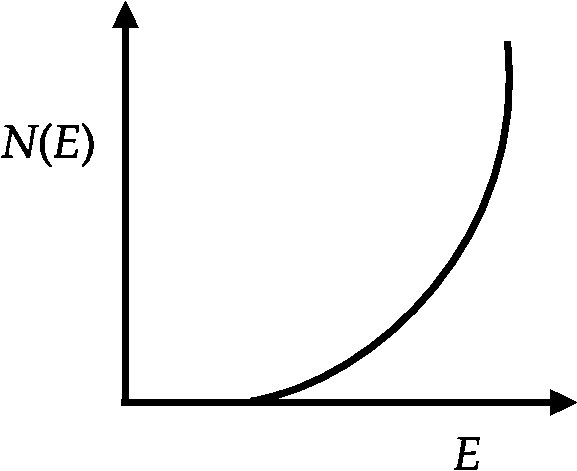
\includegraphics[height=3.5cm,width=4.5cm]{SM-01}
\end{figure}
\task[\textbf{B.}] \begin{figure}[H]
	\centering
	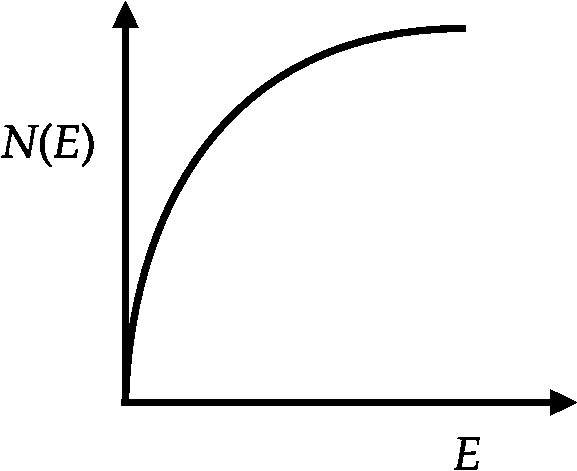
\includegraphics[height=3.5cm,width=4.5cm]{SM-02}
\end{figure}
\task[\textbf{C.}]\begin{figure}[H]
	\centering
	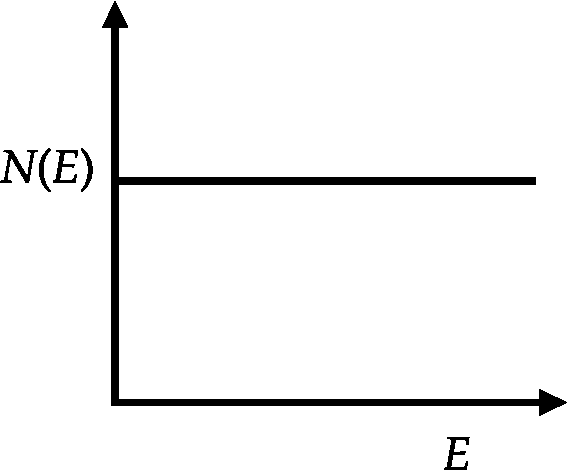
\includegraphics[height=3.5cm,width=4.5cm]{SM-03}
\end{figure} 
\task[\textbf{D.}] \begin{figure}[H]
	\centering
	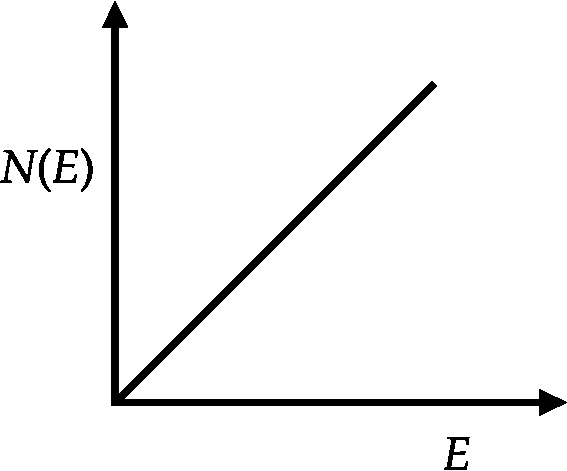
\includegraphics[height=3.5cm,width=4.5cm]{SM-04}
\end{figure}
\end{tasks}
\begin{answer}
\begin{align*}
N(E) \propto E^{0}
\end{align*}
So the correct answer is \textbf{Option (C)}
\end{answer}
	\item For a black body radiation in a cavity, photons are created and annihilated freely as a result of emission and absorption by the walls of the cavity. This is because
\begin{tasks}(1)
\task[\textbf{A.}] The chemical potential of the photons is zero
\task[\textbf{B.}] Photons obey Pauli exclusion principle
\task[\textbf{C.}] Photons are spin-1 particles
\task[\textbf{D.}] The entropy of the photons is very large
\end{tasks}
\begin{answer}
\begin{align*}
\text{The chemical potential of photon is zero}
\end{align*}
So the correct answer is \textbf{Option (A)}
\end{answer}
	\item Consider a system of $N$ non-interacting spin $-\frac{1}{2}$ particles, each having a magnetic moment $\mu$, is in a magnetic field $\vec{B}=B \hat{z} .$ If $E$ is the total energy of the system, then number of accessible microstates $\Omega$ is given by
\begin{tasks}(2)
\task[\textbf{A.}] $\Omega=\frac{N !}{\frac{1}{2}\left(N-\frac{E}{\mu B}\right) ! \frac{1}{2}\left(N+\frac{E}{\mu B}\right) !}$
\task[\textbf{B.}] $\Omega=\frac{\left(N-\frac{E}{\mu B}\right) !}{\left(N+\frac{E}{\mu B}\right) !}$
\task[\textbf{C.}] $\Omega=\frac{1}{2}\left(N-\frac{E}{\mu B}\right) ! \frac{1}{2}\left(N+\frac{E}{\mu B}\right) !$
\task[\textbf{D.}] $\Omega=\frac{N !}{\left(N+\frac{E}{\mu B}\right) !}$
\end{tasks}
\begin{answer}
\begin{align*}
\intertext{Number of microstate is ${ }^{N} C_{n_{1}}$, where $n_{1}$ is number of particle in $+\frac{1}{2}$ state and}
n_{2}&=\left(N-n_{1}\right)\text{ is number of state in }-\frac{1}{2}\text{ state.}\\
\text{	where }n_{1}&=\frac{1}{2}\left(N-\frac{E}{\mu B}\right), n_{2}=\frac{1}{2}\left(N+\frac{E}{\mu B}\right)\\
\text{So, number of microstate}=&\frac{\lfloor N}{\frac{1}{2}\left(N-\frac{E}{\mu B}\right) \mid \frac{1}{2}\left(N+\frac{E}{\mu B}\right)}
\end{align*}
\end{answer}
	\item A collection of $N$ two-level systems with energies 0 and $E>0$ is in thermal
	equilibrium at temperature $T$. For $T \rightarrow \infty$, the specific heat approaches to,
\begin{tasks}(4)
\task[\textbf{A.}] 0
\task[\textbf{B.}] $N k_{B}$
\task[\textbf{C.}] $\frac{3 N k_{B}}{2}$
\task[\textbf{D.}] $\infty$
\end{tasks}
\begin{answer}
\begin{align*}
Z&=\sum e^{-\beta E_{i}}=e^{-\beta \times 0}+e^{-\beta E_{i}} \Rightarrow Z\\&=1+e^{-\beta E} \Rightarrow \ln z\\&=\ln \left(1+e^{-\beta E}\right)\\
U&=\langle E\rangle=-\frac{\partial}{\partial \beta} \ln z\\&=-\frac{\partial}{\partial \beta} \ln \left(1+e^{-\beta E}\right)\\&=-\frac{1}{1+e^{-\beta E}} \times e^{-\beta E}(-E)\\&=\frac{E e^{-\beta E}}{1+e^{-\beta E}}\\
\text{Now},\left(\frac{\partial U}{\partial T}\right)_{V}&=C_{V}\\
&=\frac{\partial}{\partial T}\left(\frac{E e^{-\frac{E}{k T}}}{1+e^{-\frac{E}{k T}}}\right)\\
\Rightarrow C_{V}&=\frac{\left(\frac{E^{2}}{k T^{2}} e^{\frac{-E}{k T}}+\frac{E^{2}}{k T^{2}} e^{\frac{-2 E}{k T}}-\frac{E^{2}}{k T^{2}} e^{\frac{-2 E}{k T}}\right)}{\left(1+e^{\frac{-E}{k T}}\right)^{2}} \Rightarrow C_{V}\\
&=\left.\frac{\frac{E^{2}}{k T^{2}} e^{\frac{-E}{k T}}}{\left(1+e^{\frac{-E}{k T}}\right)^{2}} \Rightarrow C_{V}\right|_{T \rightarrow \infty}=0
\end{align*}
So the correct answer is \textbf{Option (A)}
\end{answer}
\item 	Consider a system of two particles $A$ and $B$. Each particle can occupy one of three possible quantum states $|1\rangle,|2\rangle$ and $|3\rangle$. The ratio of the probability that the two particles
are in the same state to the probability that the two particles are in different states is calculated for bosons and classical (Maxwell-Boltzmann) particles. They are respectively
\begin{tasks}(4)
\task[\textbf{A.}] 1,0
\task[\textbf{B.}]  $\frac{1}{2}, 1$
\task[\textbf{C.}] $1, \frac{1}{2}$
\task[\textbf{D.}] $0, \frac{1}{2}$
\end{tasks}
\begin{answer}
For two particle in same state:\\
\begin{figure}[H]
	\centering
	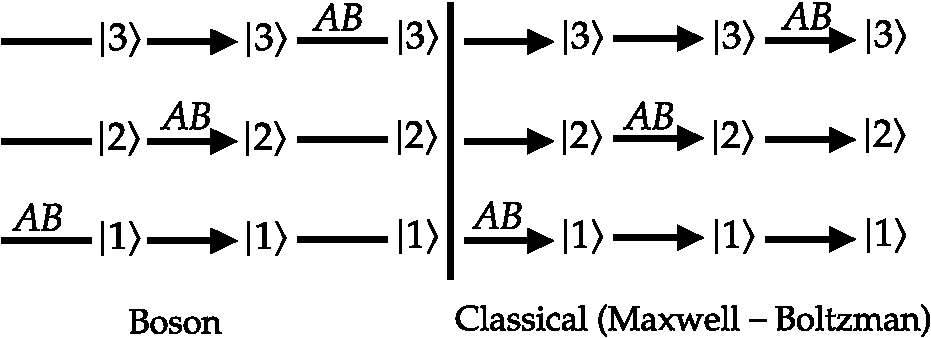
\includegraphics[height=3cm,width=8cm]{CM-20}
\end{figure}
\begin{align*}
\text{Probability ratio: }&\frac{1 / 3}{1 / 3}=1
\end{align*}
For two particle in different state;
\begin{figure}[H]
	\centering
	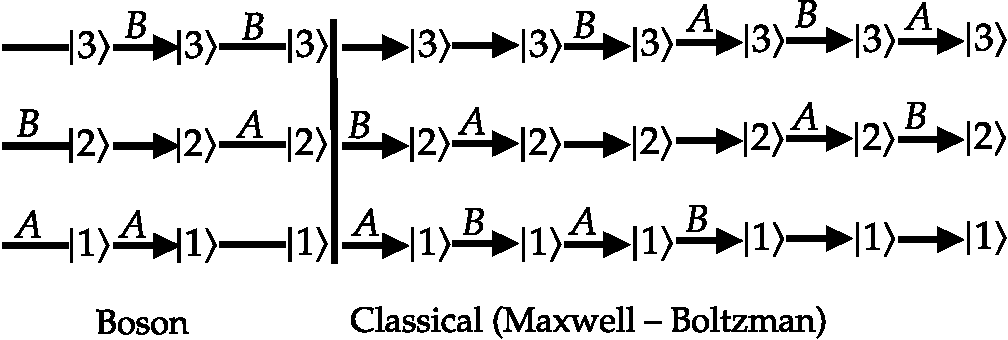
\includegraphics[height=3cm,width=11cm]{CM-21}
\end{figure}
\begin{align*}
\text{Probability ratio: }&\frac{1 / 3}{2 / 3}=\frac{1}{2}
\end{align*}
So the correct answer is \textbf{Option (C)}
\end{answer}
	\item Consider three situations of 4 particles in one dimensional box of width $L$ with hard walls. In case (i), the particles are fermions, in case (ii) they are bosons, and in case (iii) they are classical. If the total ground state energy of the four particles in these three cases are $E_{F}, E_{B}$ and $E_{c l}$ respectively, which of the following is true?
\begin{tasks}(2)
\task[\textbf{A.}] $E_{F}=E_{B}=E_{c l}$
\task[\textbf{B.}] $E_{F}>E_{B}=E_{c l}$
\task[\textbf{C.}] $E_{F}<E_{B}<E_{c l}$
\task[\textbf{D.}] $E_{F}>E_{B}>E_{c l}$
\end{tasks}
\begin{answer}
\begin{align*}
\intertext{For fermions, in 1-D box of width $L$, the ground state energy for single particle is written as,}
\frac{\pi^{2} \hbar^{2}}{2 m l^{2}}&=\epsilon_{0}\\
\Rightarrow 1 \times \in_{0}+1 \times 4 \in_{0}+1 \times 9 \in_{0}+1 \times 16 \in_{0}&=30 \in_{0}\\
\text{ For Boson }&=4 \times \epsilon_{0},\\\text{ For Maxwell }&=4 \times \epsilon_{0}\\
E_{F}>E_{B}&=E_{c l}
\end{align*}
So the correct answer is \textbf{Option (B)}
\end{answer}
	\item A monoatomic gas consists of atoms with two internal energy levels, ground state $E_{0}=0$ and an excited state $E_{1}=E$. The specific heat of the gas is given by
\begin{tasks}(2)
\task[\textbf{A.}] $\frac{3}{2} k$
\task[\textbf{B.}] $\frac{E^{2} e^{E / k T}}{k T^{2}\left(1+e^{E / k T}\right)^{2}}$
\task[\textbf{C.}] $\frac{3}{2} k+\frac{E^{2} e^{E / k T}}{k T^{2}\left(1+e^{E / k T}\right)^{2}}$
\task[\textbf{D.}] $\frac{3}{2} k-\frac{E^{2} e^{E / k T}}{k T^{2}\left(1+e^{E / k T}\right)^{2}}$
\end{tasks}
\begin{answer}
\begin{align*}
E_{0}&=0, \quad E_{1}=E\\
\text{Then partition function is}\\
z&=\sum e^{-\beta E_{i}} \Rightarrow z\\&=e^{-\beta \times 0}+e^{-\beta E} \Rightarrow \ln z\\&=\ln \left(1+e^{-\beta E_{1}}\right)\\
U&=\langle E\rangle=\frac{-\partial}{\partial \beta} \ln z\\&=-\frac{\partial}{\partial \beta} \ln \left(1+e^{-\beta E}\right)\\&=-\frac{1}{\left(1+e^{-\beta E}\right)}(-E) e^{-\beta E}\\&=\frac{E e^{-\beta E}}{1+e^{-\beta E}} \quad\left[\because \beta=k_{B} T\right]\\
\left(\frac{\partial U}{\partial T}\right)_{v}=C_{V}&=\frac{\left(1+e^{-\frac{E}{k_{B} T}}\right) E . e^{-\frac{E}{k_{B} T}} \cdot\left(\frac{E}{k_{B} T^{2}}\right)-E e^{-\frac{E}{k_{B} T}} \cdot e^{-\frac{E}{k_{B} T}}\left(\frac{E}{k_{B} T^{2}}\right)}{\left(1+e^{-\frac{E}{k_{B} T}}\right)^{2}}\\
C_{V}&=\frac{\frac{E^{2}}{k_{B} T^{2}} e^{-\frac{E}{k_{\mathrm{B}} T}}+\frac{E^{2}}{k_{B} T^{2}} e^{-\frac{2 E}{k_{\mathrm{B}} T}}-\frac{E^{2}}{k_{B} T^{2}} e^{-\frac{2 E}{k_{\mathrm{B}} T}}}{\left(1+e^{-\frac{E}{k_{\mathrm{B}} T}}\right)^{2}}\\&=\frac{E^{2} e^{-\frac{E}{k_{\mathrm{B}} T}}}{k_{B} T^{2}\left(1+e^{-\frac{E}{k_{\mathrm{B}} T}}\right)^{2}}\\&=\frac{E^{2} e^{\frac{E}{k_{\mathrm{B}} T}}}{k_{B} T^{2}\left(1+e^{\frac{E}{k_{\mathrm{B}} T}}\right)^{2}}\\
\text{If gas will classically allowed, then }C_{V}&=\frac{3}{2} k_{B}\\
\text{	and quantum mechanically, }C_{V}&=\frac{E^{2} e^{\frac{E}{k_{B} T}}}{k_{B} T^{2}\left(1+e^{\frac{E}{k_{B} T}}\right)^{2}}\\
\therefore \quad C_{V}&=\frac{3}{2} k_{B}+\frac{E^{2} e^{E / k T}}{k T^{2}\left(1+e^{E / k T}\right)^{2}}
\end{align*}
So the correct answer is \textbf{Option (C)}
\end{answer}
	\item The number of ways of distributing 11 indistinguishable bosons in 3 different energy levels is
	\begin{answer}
		Solution: $n=11 \quad g=3$
		$$
		w=\frac{\mid n+g-1}{\lfloor n \mid g-1}=\frac{\mid 11+3-1}{\lfloor 11\lfloor 2}=\frac{\lfloor 13}{\lfloor 11 \lfloor 2}
		$$
	\end{answer}
	\item The Fermi energy in copper is $7.04 \mathrm{eV}$. Compare the approximate average energy of the free electrons in copper at room temperature $(k T=0.025 \mathrm{eV})$ with their average energy if they followed Maxwell-Boltzmann statistics.
	\begin{answer}
		\begin{align*}
		\bar{\epsilon}=\epsilon_{\mathrm{F}}\left[ 1+\frac{5\pi^2}{12}\left( \frac{k_{B}T}{\epsilon_{\mathrm{F}}}\right)^2\right]\\
		=7.04\left[1+\frac{5\pi^2}{12}(\frac{0.025}{7.04})^2\right]\\ 
		=7.0403647eV\\
		\bar{E}=\frac{3}{2}kT\\
		=\frac{3}{2}\times 0.025ev\\
		=0.0375eV	
		\end{align*}
	\end{answer}
	\item Consider a linear collection of $N$ independent spin $1 / 2$ particles, each at a fixed location. The entropy of this system is $(k$ is the Boltzmann constant $)$
	\begin{answer}
		The number of microstates for a particle with spin $S=2 S+1$\\
		Therefore, total number of accessible microstates for $N$ independent spins $=(2 S+1)^{N}=\Omega$.\\
		Now, entropy $\equiv k_{B} \ln \Omega=k_{B} \ln \left[(2 S+1)^{N}\right]$\\
		Putting $S=1 / 2$, we have\\
		Entropy $=k_{B} \ln \left[(1+1)^{N}\right]=N k_{B} \ln 2$
	\end{answer}
	
	
	
	
	
	
	
	
	
\end{enumerate}